\documentclass[aps,prl,groupedaddress]{revtex4-1}  % One column - tight
%\documentclass[aps,prl,preprint,groupedaddress]{revtex4-1}  % One column - spread
%\documentclass[aps,prl,reprint,groupedaddress]{revtex4-1}  % Two column
%\documentclass[aps,prl,preprint,superscriptaddress]{revtex4-1}
%\documentclass[aps,prl,reprint,groupedaddress]{revtex4-1}

% Use the \preprint command to place your local institutional report
% number in the upper righthand corner of the title page in preprint mode.
% Multiple \preprint commands are allowed.
% Use the 'preprintnumbers' class option to override journal defaults
% to display numbers if necessary
%\preprint{}

% You should use BibTeX and apsrev.bst for references
% Choosing a journal automatically selects the correct APS
% BibTeX style file (bst file), so only uncomment the line
% below if necessary.
%\bibliographystyle{apsrev4-1}

% % % % % % % % % % % % Noam% % % % % % % % % % % % 
% Added preamble commands:
\usepackage[utf8]{inputenc}
\usepackage{array}
\usepackage{mathrsfs}
\usepackage{multirow}
\usepackage{amsmath}
\usepackage{graphicx}
\graphicspath{{Part3/}{Part3/f25_sdpfk/}{figures/phase_diagram/}{figures/levels_scheme/}{figures/decomposition/}{figures/phase_diagram/}{figures/energies_transitions_ratios/}}
\usepackage[unicode=true,pdfusetitle,bookmarks=true,bookmarksnumbered=false,bookmarksopen=false,
 breaklinks=false,pdfborder={0 0 1},backref=false,colorlinks=false]{hyperref}
%%%%%%%%%%%%%%%%%%%%%%%%%%%%%% User specified LaTeX commands.
\usepackage{braket}
%\usepackage[enable]{todonotes}
\hypersetup{colorlinks=True,urlcolor=blue,linkcolor=blue,citecolor=blue,filecolor=black}
\usepackage[caption=false]{subfig}
% Extra commands
%\usepackage{lmodern}
%\usepackage[T1]{fontenc}
%\setcounter{secnumdepth}{3}
%\usepackage{color}
%\usepackage{float}
%\usepackage{mathtools}
%\usepackage{amssymb}
%\usepackage{breakurl}

%\usepackage{pslatex}  % Change font style.
%\renewcommand{\arraystretch}{1.5}  % Widens rows in Tables
%\setlength{\extrarowheight}{2pt}   % Widens rows in Tables

\makeatletter

%%%%%%%%%%%%%%%%%%%%%%%%%%%%%% LyX specific LaTeX commands.
%% Because html converters don't know tabularnewline
\providecommand{\tabularnewline}{\\}
%% A simple dot to overcome graphicx limitations
\newcommand{\lyxdot}{.}

\makeatother

\begin{document}

%Title of paper
\title{Shell-model project for Nuclear Talent course - Solutions}

% repeat the \author .. \affiliation  etc. as needed
% \email, \thanks, \homepage, \altaffiliation all apply to the current
% author. Explanatory text should go in the []'s, actual e-mail
% address or url should go in the {}'s for \email and \homepage.
% Please use the appropriate macro foreach each type of information

% \affiliation command applies to all authors since the last
% \affiliation command. The \affiliation command should follow the
% other information
% \affiliation can be followed by \email, \homepage, \thanks as well.
\author{Group 1}
%\email[]{Your e-mail address}
%\homepage[]{Your web page}
%\thanks{}
%\altaffiliation{}
\affiliation{}

%Collaboration name if desired (requires use of superscriptaddress
%option in \documentclass). \noaffiliation is required (may also be
%used with the \author command).
%\collaboration can be followed by \email, \homepage, \thanks as well.
%\collaboration{}
%\noaffiliation

\date{\today}

\begin{abstract}
% insert abstract here
\end{abstract}

% insert suggested PACS numbers in braces on next line
\pacs{}
% insert suggested keywords - APS authors don't need to do this
%\keywords{}

%\maketitle must follow title, authors, abstract, \pacs, and \keywords
\maketitle
\section{Part 3 - N. Gavrielov}

\subsection{$^{18}$O and $^{18}$F}

\subsection{NushellX for $^{18-28}$O}

\subsection{NushellX for $^{18-29}$F}
\subsubsection{$^{30-31}$F}
We test different effective interactions in $sd-pf$ shell using the $0f_{7/2}$ and $1p_{3/2}$ orbits.

\subsection{Negative Parity for $^{25}$O and $^{25}$F}
In the $sd$ shell, all orbits are with positive parity and therefore negative parity states can not be calculated. Extending to the $sd-pf$ shell one might encounter some, however using the SDPF-K interaction, taking an $^{16}$O core for the protons and freezing 12 neutrons in the $sd$ shell (12 particle filling all the $sd$ orbits) with extra 5 neutrons at the $0f_{7/2}$ and $1p_{3/2}$ orbits we still do not obtain negative parity states. \textbf{This might need some further explanation}.
\begin{figure}[h]
\centering
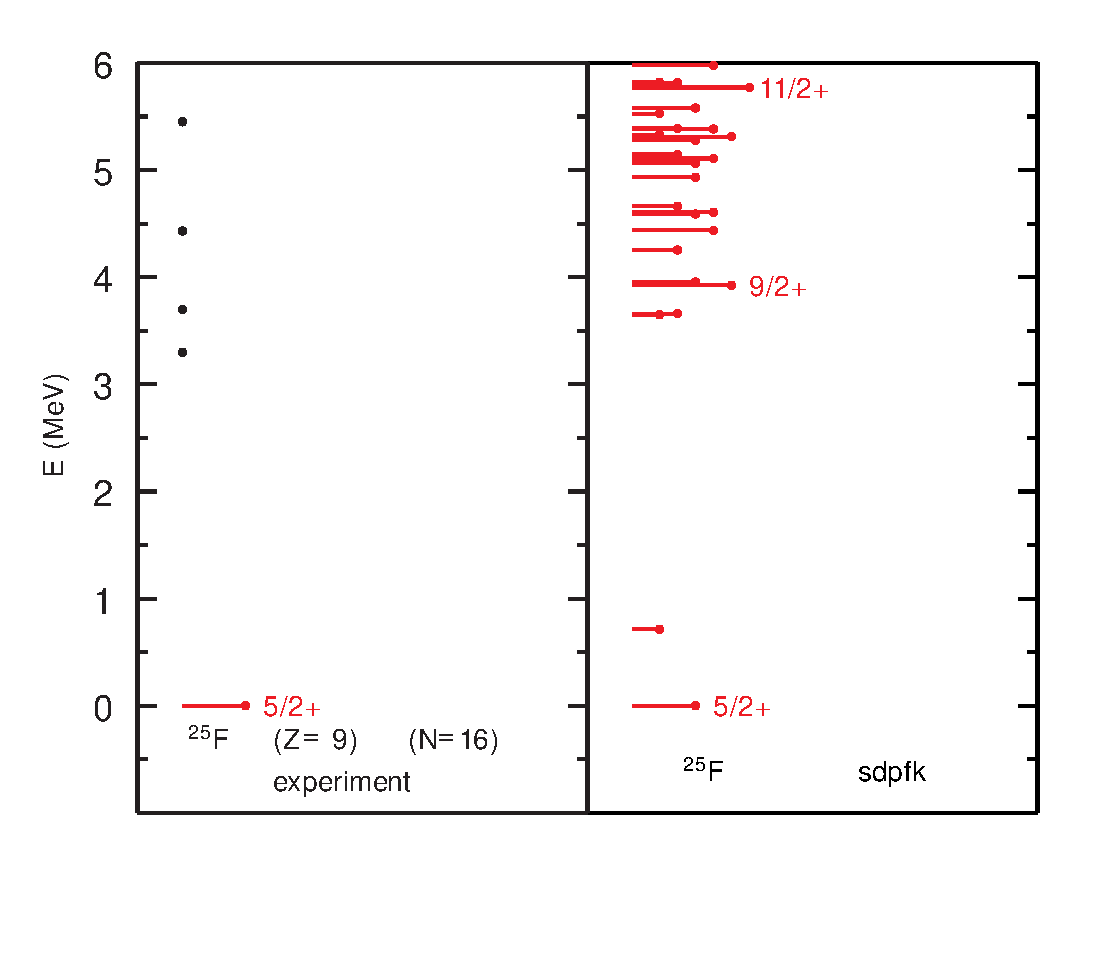
\includegraphics[width=0.45\linewidth]{f_25k.eps}
\caption{test}
\label{fig:F-25-SDPF-K}
\end{figure}

\bibliography{/home/noam/Desktop/Physics/Articles/library.bib}
\end{document}


